\subsection{Frequency tables}
A frequency distribution is a table that shows ``classes`` or ``intervals`` of data 
entries with a count of the number of entries in each class. The frequency $f$ of 
a class is the number of data entries in the class. Each class will have a 
``lower limit``' and an ``upper limit`` which can be interpreted as the 
lowest and highest numbers in each class. The “class width” is defined as the 
distance between the lower limits of consecutive classes. Before constructing a 
frequency table, some consideration should be given about the range of values in 
the dataset. In situations where there are to many class intervals, the likelihood 
of reducing the bulkiness of the data is highly unlikely. On the other hand, if 
the total number of classes is minimal, then the shape of the distribution itself 
cannot be successfully determined. Generally, for most datasets 6-14 intervals 
is considered an ideal benchmark \cite{c7}. However, this should not be interpreted as the 
defacto standard as a lot depends on the dataset itself. With that being said, 
the following are a few general guidelines one can follow when constructing a 
frequency table. 

\begin{enumerate}
    \item The ideal number of classes can be determined or approximated by the 
    formulas: 
    \begin{align}
        C = 1 + 3.3\log{n} \label{sturges}
    \end{align}
    \begin{align}
        C = \sqrt{n} \label{rootChoice}
    \end{align}
    where $n$ is the total number of observations in the dataset. Formally, 
    equation \ref{sturges} is known as Sturge's Rule while equation \ref{rootChoice}
    is known as the Square Root Choice Rule. 
    \item Calculate the range of the data by finding the minimum and maximum data 
    values. 
    \item  Using the range, find the width of the classes which can be determined
    using the formula:
    \begin{equation}
        \mbox{Class Width} = \frac{\mbox{range}}{\mbox{number of classes}}
    \end{equation}
    \item To find the class limits use the minimum data entry as the lower limit 
    of the first class. Then to get the lower limit of the next class, add the 
    class width. Continue until you reach the last class. Then find the upper 
    limits of each class.
\end{enumerate}

\begin{table}[!ht]
    \centering
    \caption{Age Frequency's for Males}
    \scalebox{.9} {
        \begin{tabular}{c@{\hspace*{1.5cm}}c@{\hspace*{0cm}}l}
            \hline
            Age & Frequency \\ 
            \hline
            17 & 1 \\			
            20 & 2 \\			
            21 & 6 \\			
            22 & 5 \\			
            23 & 6 \\			
            24 & 5 \\			
            25 & 9 \\			
            26 & 15 \\			
            27 & 18 \\			
            28 & 17 \\	
            \hline
            \multicolumn{2}{l}{*Sample of a simple frequency table.}
        \end{tabular}
    }
    \label{table:oodbmsTerminology}
\end{table}

The main advantage of a frequency table is their ability to quickly reveal 
outliers and even significant trends within a dataset with not much more than 
a quick inspection. However, the milage might vary on this as extremely 
large datasets might make it difficult for a simple inspection to be enough. This 
leads to a major disadvantage of a frequency table where they are not always 
readily apparent depending on the dataset size. For instance, there may be situations 
where unless other visualization graphs are used, characteristics such as skewness 
are not inherently obvious.   

\subsection{Frequency Distribution Graphs}
A frequency distribution graph is a diagrammatic illustration of the information 
in the frequency table. 

\subsubsection{Histogram}
A histogram is a graphical representation of the variable of interest in the 
$X$ axis versus the number of observations (frequency) in the $Y$ axis. Percentages 
can also be used if the goal is to compare two histograms with a different number of 
categories. Typically, a histogram is used to depict the frequency when data is 
measured against an interval or ratio scale. They are great to highlight skewness
and work well with large ranges in a dataset. Coincidentally, there is a striking
resemblance between a bar chart and a histogram. However, they are nothing alike 
with three important distinctions between them to be aware of. First off, in a histogram there 
are no gaps between bars as the variable is continuous. In a bar chart, oftentimes 
there is a noticeable amount of space between the bars depending on the aspect
ratio. Secondly, in histograms the width of the bars have a meaning and do not 
need to be of equal length as this depends on the class interval. Whereas in a bar 
chart all the bars widths are equal in length. Finally, in histograms the area 
of each bar corresponds to the frequency whereas in a bar chart, it is the height \cite{c10}. 
Figure \ref{figure:histogram} is an example of a histogram created in \textit{R} 
using the \textit{ggplot2} library. Unfortunately, this figure also exposes a major 
weakness when interpreting histograms. It is extremely difficult and practically 
impossible to extract the exact amount of ``input`` unless the frequencies are listed 
above the bars. Luckily, there is a version of a histogram that does just this 
called a frequency histogram should that feature become a necessity. 

\begin{figure}[!ht]
    \centering
        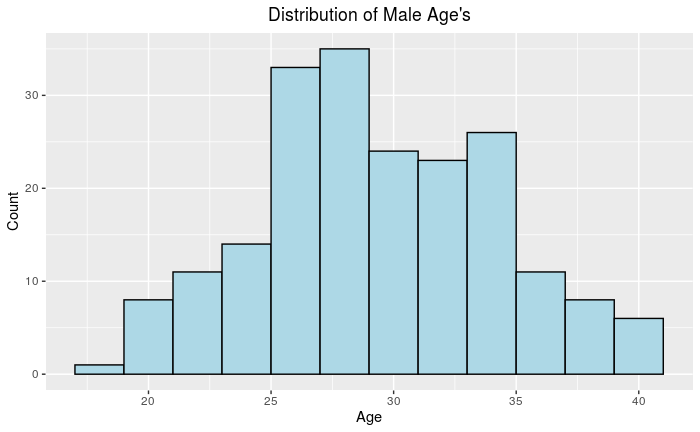
\includegraphics[height=5cm]{figures/histogram.png}
    \caption{Histogram built in R using the ggplot2 library.}
    \label{figure:histogram}
\end{figure} 

\subsubsection{Frequency Polygon}
A frequency polygon is very similar to a histogram. In fact, they are almost 
identical but differ in that frequency polygons are used to compare sets of data or 
to display a cumulative frequency distribution. A cumulative distribution is a 
form of a frequency distribution that represents the sum of a class and all the
classes below it. They are extremely useful when you need to determine the frequency 
up to a specific threshold or to easily compare two frequency distributions quickly.
Visually, there is also a slight difference where histograms use rectangles 
while a frequency polygon resembles a line graph. Constructing a frequency polygon 
is done by connecting all midpoints of the top of the bars in a histogram by a 
straight line and then removing the bars. Furthermore, when the total frequency is large 
and the class intervals are narrow, the frequency polygon has the tendency to become 
a smooth curve which is formally known as the ``frequency curve``. Figure \ref{figure:freq_polygon}
is an example of a frequency polygon built using the same tools as the histogram. The 
main advantage of a frequency polygon involves their ability to show central 
tendencies and dispersion clearly on large datasets. However, given their close 
relationship to histograms, unsurprisingly frequency polygons share many of their 
downsides too such as the loss of details on relative numbers and proportions. 

\begin{figure}[!ht]
    \centering
        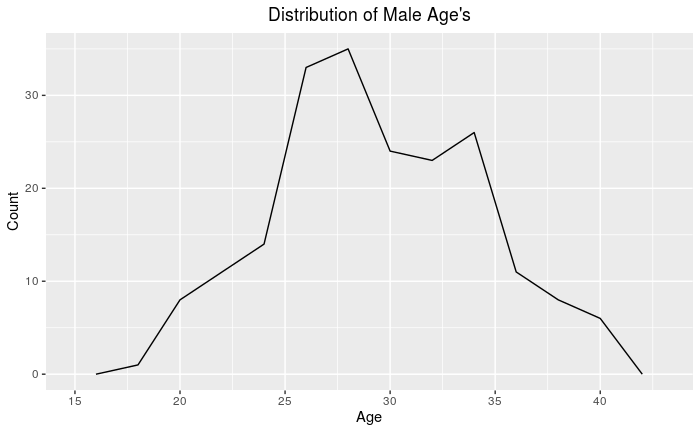
\includegraphics[height=5cm]{figures/freq_polygon.png}
    \caption{Frequency Polygon built in R using the ggplot2 library.}
    \label{figure:freq_polygon}
\end{figure}  

\subsubsection{Box and Whisker Plot}
First described by John Tukey in 1977, the box and whisker plot is a histogram
type visualization that can be used to illustrate frequency distributions \cite{c10}. Constructing
a box and whisker plot requires a vertical or horizontal rectangle (box) where the 
ends are used to represent the upper and lower quartiles. The middle 50\% of observations 
is represented by the box itself and the length of the box indicates the variability 
of the data while the line inside represents the median. Interestingly enough, 
the position of the median visually indicates whether or not the dataset is skewed. 
In fact, for instances where the median is closer to the upper quartile we say that 
the dataset is positively skewed and for instances where the median is closer to 
the lower quartile we say it is negatively skewed. 
The lines outside the box on either side are known as whiskers and each whisker 
is roughly 1.5 times the length of the box. The ends of whiskers are called the 
``inner fence``' and any data point beyond its boundary is considered an outlier. 
Furthermore, the dataset distribution plays a role in the length of the whiskers 
where if symmetrical the whiskers will be of equal length. But if the dataset 
is sparse on one side, the corresponding side whisker will be short. The ``outer fence``
which is roughly defined as the section farthest away from the whiskers is at a 
distance of three times the IQR on either side of the box. The reasoning behind 
having the inner and outer fence at 1.5 and 3 times the IQR, is due to the assumption 
that 95\% of observations fall within 1.5 times the IQR, and another 99\% for 3 
times the IQR \cite{c10}. The biggest advantage of the box and whisker plot is its ability 
to handle large amounts of data and clearly highlight outliers as illustrated in 
Figure \ref{figure:box_and_whisker}. However, the biggest downside is its inability to
to retain the exact values and details of a distribution. Unfortunately, this type
of visualization is meant to only show a simple summary of the distribution and
should be used in combination with other visualizations when analyzing a dataset.

\begin{figure}[!ht]
    \centering
        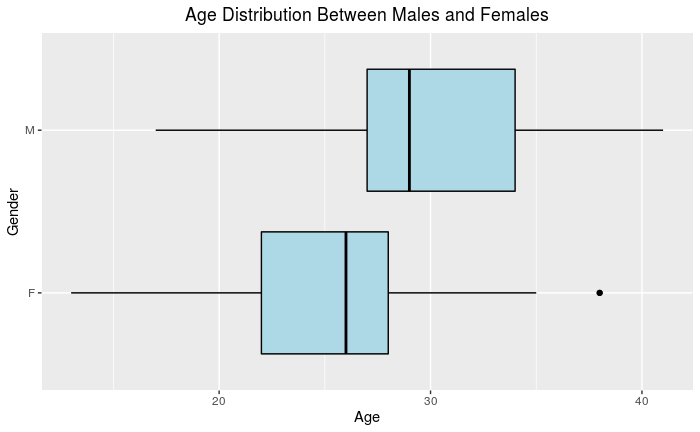
\includegraphics[height=5cm]{figures/box_and_whisker.png}
    \caption{Box and Whisker Plot built in R using the ggplot2 library.}
    \label{figure:box_and_whisker}
\end{figure} 

\subsubsection{Bubble Chart}
A Bubble chart is a type of multi-variable graph that can be viewed as a variation 
of the Scatterplot. In Bubble charts, the additional dimension of the data is represented 
in the size of the bubble. Much like a Scatterplot, Bubble charts are plotted on 
a cartesian coordinate system where the $X$ and $Y$ axis represent separate variables. 
However, unlike a Scatterplot the Bubble chart assigns a label or category for
each point. Colors can also be used to distinguish between categories or used to 
represent an additional data variable. It is also possible to convey time in the
Bubble chart by either having it as a variable on one of the axis or by animating 
the data variables changing over time through the use of software tools. In practice,
Bubble charts are used to compare and show the relationships between categorized 
circles, through the use of positioning and proportions. The overall picture of 
Bubble charts can be used to analyze for patterns and correlations. But if to many bubbles 
are used it can make the chart difficult to read and comprehend as illustrated in 
Figure \ref{figure:bubble_chart}. Therefore, Bubble charts should be considered as
having a limited size capacity when constructed. However, this is mostly true for 
static versions of Bubble charts as this limitation is somewhat nonexistent for 
their interactive counterparts. 

\begin{figure}[!ht]
    \centering
    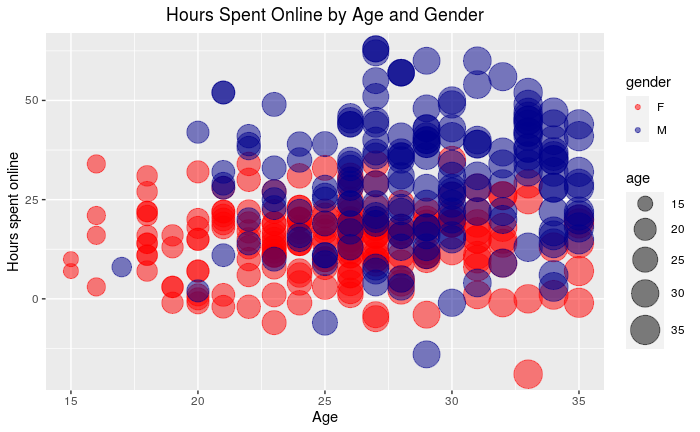
\includegraphics[height=5cm]{figures/bubble_chart.png}
    \caption{Bubble chart built in R using the ggplot2 library.}
    \label{figure:bubble_chart}
\end{figure} 

When built with software tools, clicking or hovering over bubbles to display hidden 
information or having an option to reorganize and filter out grouped categories 
helps to increase the number of potential bubbles in the chart. Furthermore, to 
avoid misinterpretations of the bubbles their size should be based on the area of 
a circle, not the radius or diameter. This is to avoid the side effect of the circles 
changing exponentially and unintentionally tricking the human eye into interpreting 
drastic changes in the dataset that are potentially not true.

\subsubsection{Multi-set Bar Chart}
Multi-set Bar Charts which can also be refereed to as Grouped Bar Charts or Clustered 
Bar Charts are a variation of traditional Bar Charts. They are primarily used when 
two or more data series are plotted side-by-side and grouped together under categories, 
all on the same axis. Like a Bar Chart, the length of each bar is used to show 
discrete, numerical comparisons between the categories. Each data series is assigned 
an individual color, in order to distinguish amongst the categories. Furthermore, 
each group of bars is spaced apart to increase visual comprehension. Multi-set 
Bar charts are best suited to compare grouped variables or categories to other 
groups with those same variables or category types. The downside of Multi-set Bar 
charts is that they become harder to comprehend as more bars are added into a 
group.
